\section{Sensitivity Analysis}

An important aspect of any fuel cycle transition scenario
is the accrual of fissile materials for new reactor deployment.
The collaborative strategy makes a transition possible 
from the perspective of material availability,
but the aggressive transition demands a significant increase in reprocessing capacity.

We explored the impact of two key variables, the lifetime of French \glspl{LWR} and the
breeding ratio of \gls{ASTRID} reactors. The range over which we varied these parameters (\cref{tab:sen_par})
sought to capture the full span of their uncertainty.

\begin{table}[h]
    \centering
    \begin{tabularx}{\textwidth}{lbb}
        \hline
        \textbf{Parameter} & \textbf{Default} & \textbf{Values} \\
        \hline
        Breeding Ratio of \glspl{ASTRID} & 1.08 & 1.11, 1.15, 1.18 \\ 
        Lifetime of French \glspl{LWR} [years] & 60  & 65, 70, 80 \\
        \hline
    \end{tabularx}
    \caption {Two parameters were varied for the sensitivity analysis - the 
              lifetime of French \glspl{LWR} and the breeding ratio of \glspl{ASTRID}.
              The parameters are increased to analyze their impact on the reprocessing
              demand for the transition.}
    \label{tab:sen_par}
\end{table}

\subsection{Breeding Ratio}

Increase in the breeding ratio of \gls{ASTRID} reactors
decreases the monthly reprocessing demand, as shown in figure \ref{fig:br_rep}.
Increase in breeding ratio also reduces the number of total \gls{UOX} \gls{UNF}
required for the transition, because the \gls{ASTRID} creates more plutonium.


\begin{figure}[htbp!]
    \begin{center}
        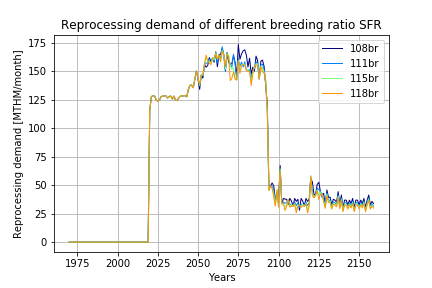
\includegraphics[scale=0.6]{./images/sensitivity/br_tot_rep.png}
    \end{center}
    \caption{Increasing the breeding ratio decreases the monthly reprocessing demand. The
             demand up to 2050 is unaffected by breeding ratio because only \gls{UOX} \gls{UNF}
             is reprocessed.}
    \label{fig:br_rep}
\end{figure}


\begin{figure}[htbp!]
    \begin{center}
        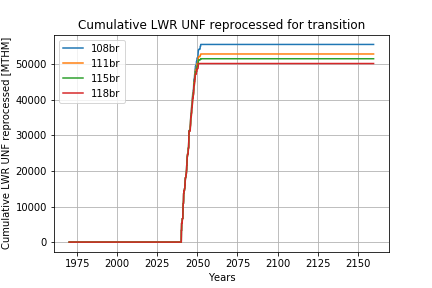
\includegraphics[scale=0.6]{./images/sensitivity/br_uox_unf_cum.png}
    \end{center}
    \caption{Increasing the breeding ratio decreases the number of total \gls{UOX} \gls{UNF}
             required. The \glspl{ASTRID} produce more plutonium, reducing the plutonium demand
             from reprocessed \gls{UOX}.}
    \label{fig:br_uox}
\end{figure}


\subsection{Lifetime Extension of French \glspl{LWR}}\label{sec:life}
Extending the lifetime of French \glspl{LWR} dramatically lowers the average
monthly \gls{UOX} reprocessing demand, since the \gls{ASTRID} deployment becomes 
delayed (shown in figure \ref{fig:pow_diff}). The plutonium demand is delayed,
 allowing the reprocessing plant more time to prepare plutonium for \gls{ASTRID} reactors. 

Figure \ref{fig:ext_uox} shows the decrease in the average monthly
\gls{UOX} reprocessing burden with increased \gls{LWR} lifetimes,
which reduces to the current capacity of the La Hague site if all the
French \glspl{LWR} extended their operation for 20 years.
Figure \ref{fig:ext_all} shows that lifetime extension has little
effect on the average total monthly reprocessing demand, because
the amount of plutonium in the \gls{ASTRID} used fuel remains the same.
The initial increase is caused by the delay of \gls{ASTRID} deployment
delaying the first \gls{ASTRID} \gls{UNF} reprocessing. The period of which
\gls{ASTRID} \gls{UNF} is reprocessed decreases, which increases
the average.

\begin{figure}[htbp!]
    \begin{center}
        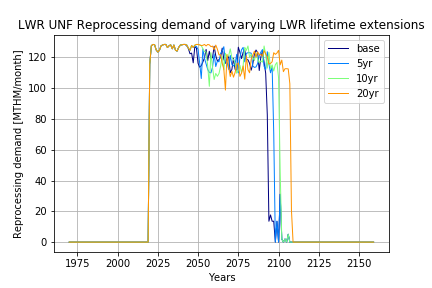
\includegraphics[scale=0.6]{./images/sensitivity/ext_uox_rep.png}
    \end{center}
    \caption{Increasing the lifetime of French \glspl{LWR} decreases the monthly
             \gls{UOX} reprocessing demand, by allowing a less aggressive transition
             to \glspl{ASTRID}.}
    \label{fig:ext_uox}
\end{figure}


\begin{figure}[htbp!]
    \begin{center}
        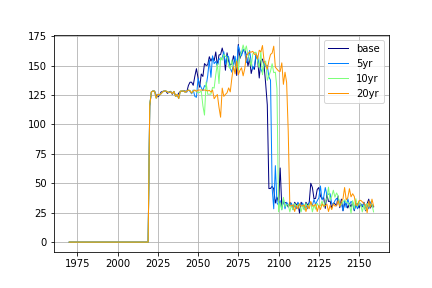
\includegraphics[scale=0.6]{./images/sensitivity/ext_tot_rep.png}
    \end{center}
    \caption{Increasing the lifetime of French \glspl{LWR} simply delays the
             reprocessing demand, and has little impact on the amount of reprocessing
             required.}
    \label{fig:ext_all}
\end{figure}


\begin{figure}[htbp!]
    \begin{center}
        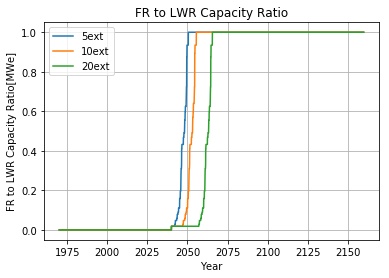
\includegraphics[height=0.25\textheight]{./images/sensitivity/pow_ratio.png}
    \end{center}
    \caption{This plot shows the ratio of \glspl{ASTRID} to \glspl{LWR} in France.
             The delay in \gls{ASTRID} deployment allows more
              time for the reprocessing plant to prepare the plutonium 
              for \gls{ASTRID} fuel production.}
    \label{fig:pow_diff}
\end{figure}
